\documentclass[12pt]{article}
\usepackage[fleqn]{amsmath}
\usepackage{amsthm,amsfonts,amssymb,braket,enumitem,minted,hyperref,cleveref,tikz}
\usetikzlibrary{shapes}

\newtheorem{theorem}{Theorem}[section]
\newtheorem{corollary}{Corollary}[theorem]
\newtheorem{lemma}[theorem]{Lemma}
\theoremstyle{definition}
\newtheorem{definition}{Definition}[section]
\newenvironment{solution}
{\renewcommand\qedsymbol{$\blacksquare$}
\begin{proof}[Solution]}
  {
\end{proof}}
\hypersetup{
  colorlinks=true,
  urlcolor=violet,
  linkcolor=blue,
}

\begin{document}

\begin{center}
  {\Large CPT\_S 223 Homework 4}
  $ $\\
  $ $\\
  \begin{tabular}{rl}
    WSU ID: & 11870028 \\
    Name: & Neal Wang \\
    Due Date: & 10 April 2025
  \end{tabular}
\end{center}

\section{Problem 1}

\begin{enumerate}[label=(\alph*)]
  \item
    ~\\
    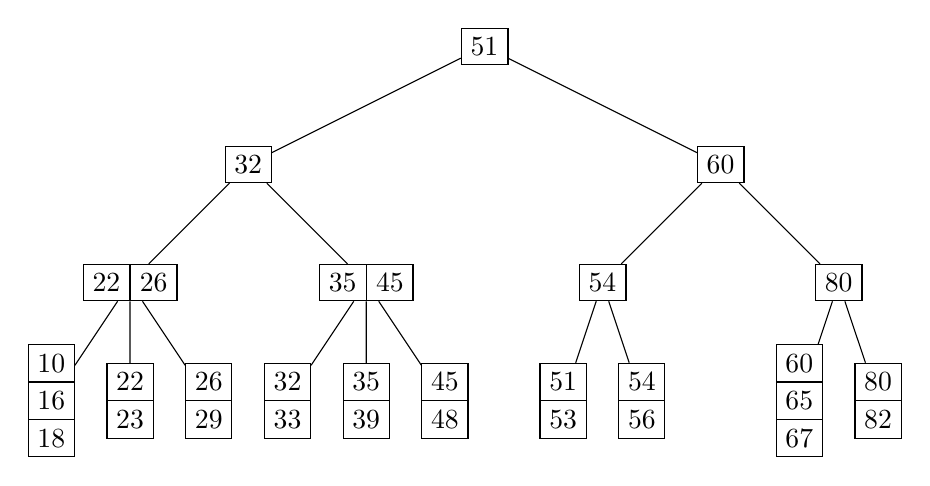
\begin{tikzpicture}
      \tikzstyle{bplus}=[
        rectangle split, rectangle split horizontal, rectangle split
        ignore empty parts, draw
      ]
      \tikzstyle{every node}=[bplus]
      \tikzstyle{level 1}=[sibling distance=60mm]
      \tikzstyle{level 2}=[sibling distance=30mm]
      \tikzstyle{level 3}=[
        sibling distance=10mm,
        every node/.style={
          rectangle split, rectangle split ignore empty parts, draw
        }
      ]
      \node{51}
      child{node{32}
        child{node{22 \nodepart{two} 26}
          child{node{10 \nodepart{two} 16 \nodepart{three} 18}}
          child{node{22 \nodepart{two} 23}}
          child{node{26 \nodepart{two} 29}}
        }
        child{node{35 \nodepart{two} 45}
          child{node{32 \nodepart{two} 33}}
          child{node{35 \nodepart{two} 39}}
          child{node{45 \nodepart{two} 48}}
        }
      }
      child{node{60}
        child{node{54}
          child{node{51 \nodepart{two} 53}}
          child{node{54 \nodepart{two} 56}}
        }
        child{node{80}
          child{node{60 \nodepart{two} 65 \nodepart{three} 67}}
          child{node{80 \nodepart{two} 82}}
        }
      };
    \end{tikzpicture}
  \item
    ~\\
    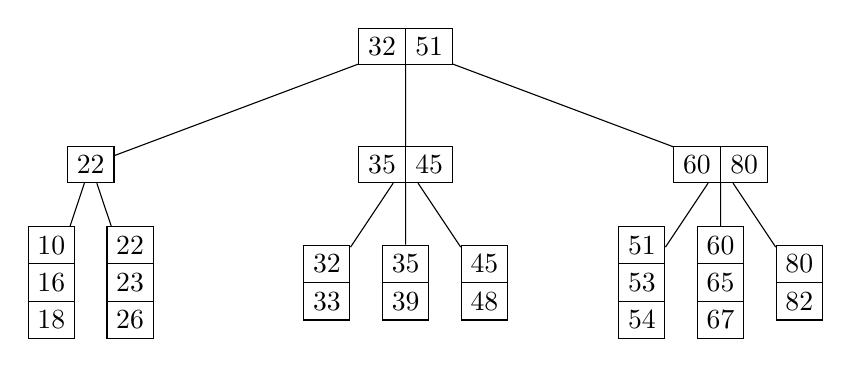
\begin{tikzpicture}
      \tikzstyle{bplus}=[
        rectangle split, rectangle split horizontal, rectangle split
        ignore empty parts, draw
      ]
      \tikzstyle{every node}=[bplus]
      \tikzstyle{level 1}=[sibling distance=40mm]
      \tikzstyle{level 2}=[
        sibling distance=10mm,
        every node/.style={
          rectangle split, rectangle split ignore empty parts, draw
        }
      ]
      \node{32 \nodepart{two} 51}
      child{node{22}
        child{node{10 \nodepart{two} 16 \nodepart{three} 18}}
        child{node{22 \nodepart{two} 23 \nodepart{three} 26}}
      }
      child{node{35 \nodepart{two} 45}
        child{node{32 \nodepart{two} 33}}
        child{node{35 \nodepart{two} 39}}
        child{node{45 \nodepart{two} 48}}
      }
      child{node{60 \nodepart{two} 80}
        child{node{51 \nodepart{two} 53 \nodepart{three} 54}}
        child{node{60 \nodepart{two} 65 \nodepart{three} 67}}
        child{node{80 \nodepart{two} 82}}
      };
    \end{tikzpicture}
\end{enumerate}

\section{Problem 2}

I would pick 101 as the initial hash table size.

7 is too small for most practical uses.

100, 27, and 525 are all composite numbers, which leads to more
clustering and collisions if a modulo hash function is used.

\section{Problem 3}

\begin{enumerate}[label=(\alph*)]
  \item
    ~\\
    \begin{tabular}{|c|c|c|c|c|c|c|}
      \hline
      0 & 1 & 2 & 3 & 4 & 5 & 6 \\ [0.5ex]
      \hline
      33, 5, 58, 2, 40 & & & 42, 14, 84 & 6 & 45 & \\
      \hline
    \end{tabular}
  \item
    ~\\
    \begin{tabular}{|c|c|c|c|c|c|c|c|c|c|c|}
      \hline
      0 & 1 & 2 & 3 & 4 & 5 & 6 & 7 & 8 & 9 & 10 \\ [0.5ex]
      \hline
      40 & 14 & 58 & 33 & 45 & & 5 & 42 & 84 & 6 & 2 \\
      \hline
    \end{tabular}
  \item
    ~\\
    \begin{tabular}{|c|c|c|c|c|c|c|c|c|c|c|}
      \hline
      0 & 1 & 2 & 3 & 4 & 5 & 6 & 7 & 8 & 9 & 10 \\ [0.5ex]
      \hline
      2 & 14 & 58 & 33 & 45 & & 5 & 42 & 84 & 40 & 6 \\
      \hline
    \end{tabular}
  \item
    ~\\
    \begin{tabular}{|c|c|c|c|c|c|c|c|c|c|c|}
      \hline
      0 & 1 & 2 & 3 & 4 & 5 & 6 & 7 & 8 & 9 & 10 \\ [0.5ex]
      \hline
      58 & 14 & & 33 & 45 & 2 & 5 & 42 & 84 & 9 & 40 \\
      \hline
    \end{tabular}
\end{enumerate}

\section{Problem 4}

The performance issue is likely due to the fact that the new hash
table is always double the size of the previous one:

\begin{minted}{c}
array.resize(2 * oldArray.size())
\end{minted}

This means that after multiple rehashes, the table size will be a
number that has divisors. This is problematic because entries that
are multiples of those divisors will keep mapping onto each other,
causing a large number of collisions.

A potential solution is to pick the the next table size to be the
smallest prime number larger than twice the current size. This can be
implemented using a
\href{https://en.wikipedia.org/wiki/Sieve_of_Eratosthenes}{sieve of
Eratosthenes}, which is what I used for
\href{https://github.com/mathletedev/cpt_s/blob/b7051f9f4cdd25d00f1a66aae65da3f2133e4883/223/assignments/pa4/src/hash_map.hpp#L57}{PA4}.

\end{document}
